\subsection{真正重建：为什么必须再检验一次}
冻结状态的GN比较把当前材料、总场和残差暂时固定。真正的非线性反演（nonlinear reconstruction）执行一步以后，这些量都会改变。还必须满足材料可行域（material feasibility constraints），并用线搜索（line search）判断新材料是否使完整非线性目标下降。因此，局部GN gap和最终材料误差（final material error）是两个不同指标。

固定的四个代表对象使用$k=8$，两种策略共享初始化$0.1+0.04i$、prior、LM schedule、实部下界$-0.5$、虚部下界0以及Armijo充分下降检验（Armijo acceptance）。每次先投影可行材料步，再从$\alpha=1$开始减半，最多24次；两条轨迹只改变切向电流空间。三组对照完成18次更新。

\begin{table}[htbp]\centering\small
\caption{完整三维材料相对误差：receiver $\to$ exchange。不是中心切片误差。}
\begin{tabular}{lrrr}\toprule
几何 / 表示&复材料&实部&虚部\\\midrule
平滑 / voxel&$0.3027\to0.2699$&$0.2811\to0.2516$&$0.7439\to0.6506$\\
近接触 / Gaussian&$0.6722\to0.6707$&$0.6810\to0.6835$&$0.4439\to0.2859$\\
shell / Gaussian&$0.6096\to0.5660$&$0.6081\to0.5651$&$0.6976\to0.6219$\\\bottomrule
\end{tabular}
\end{table}

三组复材料误差下降约10.8\%、0.22\%、7.16\%，留出测量误差（held-out data error）也下降。近接触对象尤其说明，数据拟合改善并不自动意味着材料所有分量改善：它的实部误差略升，复误差几乎中性。非对称voxel对象的exchange轨迹完成17次接受更新以后，在第18次更新前构建的receiver初始端点未通过预定法方程残差检查，故exchange轨迹停止。独立的receiver-only基线未运行；没有把最后安全状态当作完成终点，也不能据此推断未运行基线一定失败。

完整耗时（all-in wall time）包括每条轨迹自己的物理setup、anchor/pool获取、被拒绝的检查、line search和终点评价。三组耗时比是2.68、1.74、1.46；额外完整切向RHS分别为708、744、744，其中包含$Jx$初始化和$Jd$复核。这个方法的意义是用额外物理作用购买局部更新保真度，现有结果没有证明加速成像。

\begin{figure}[htbp]\centering
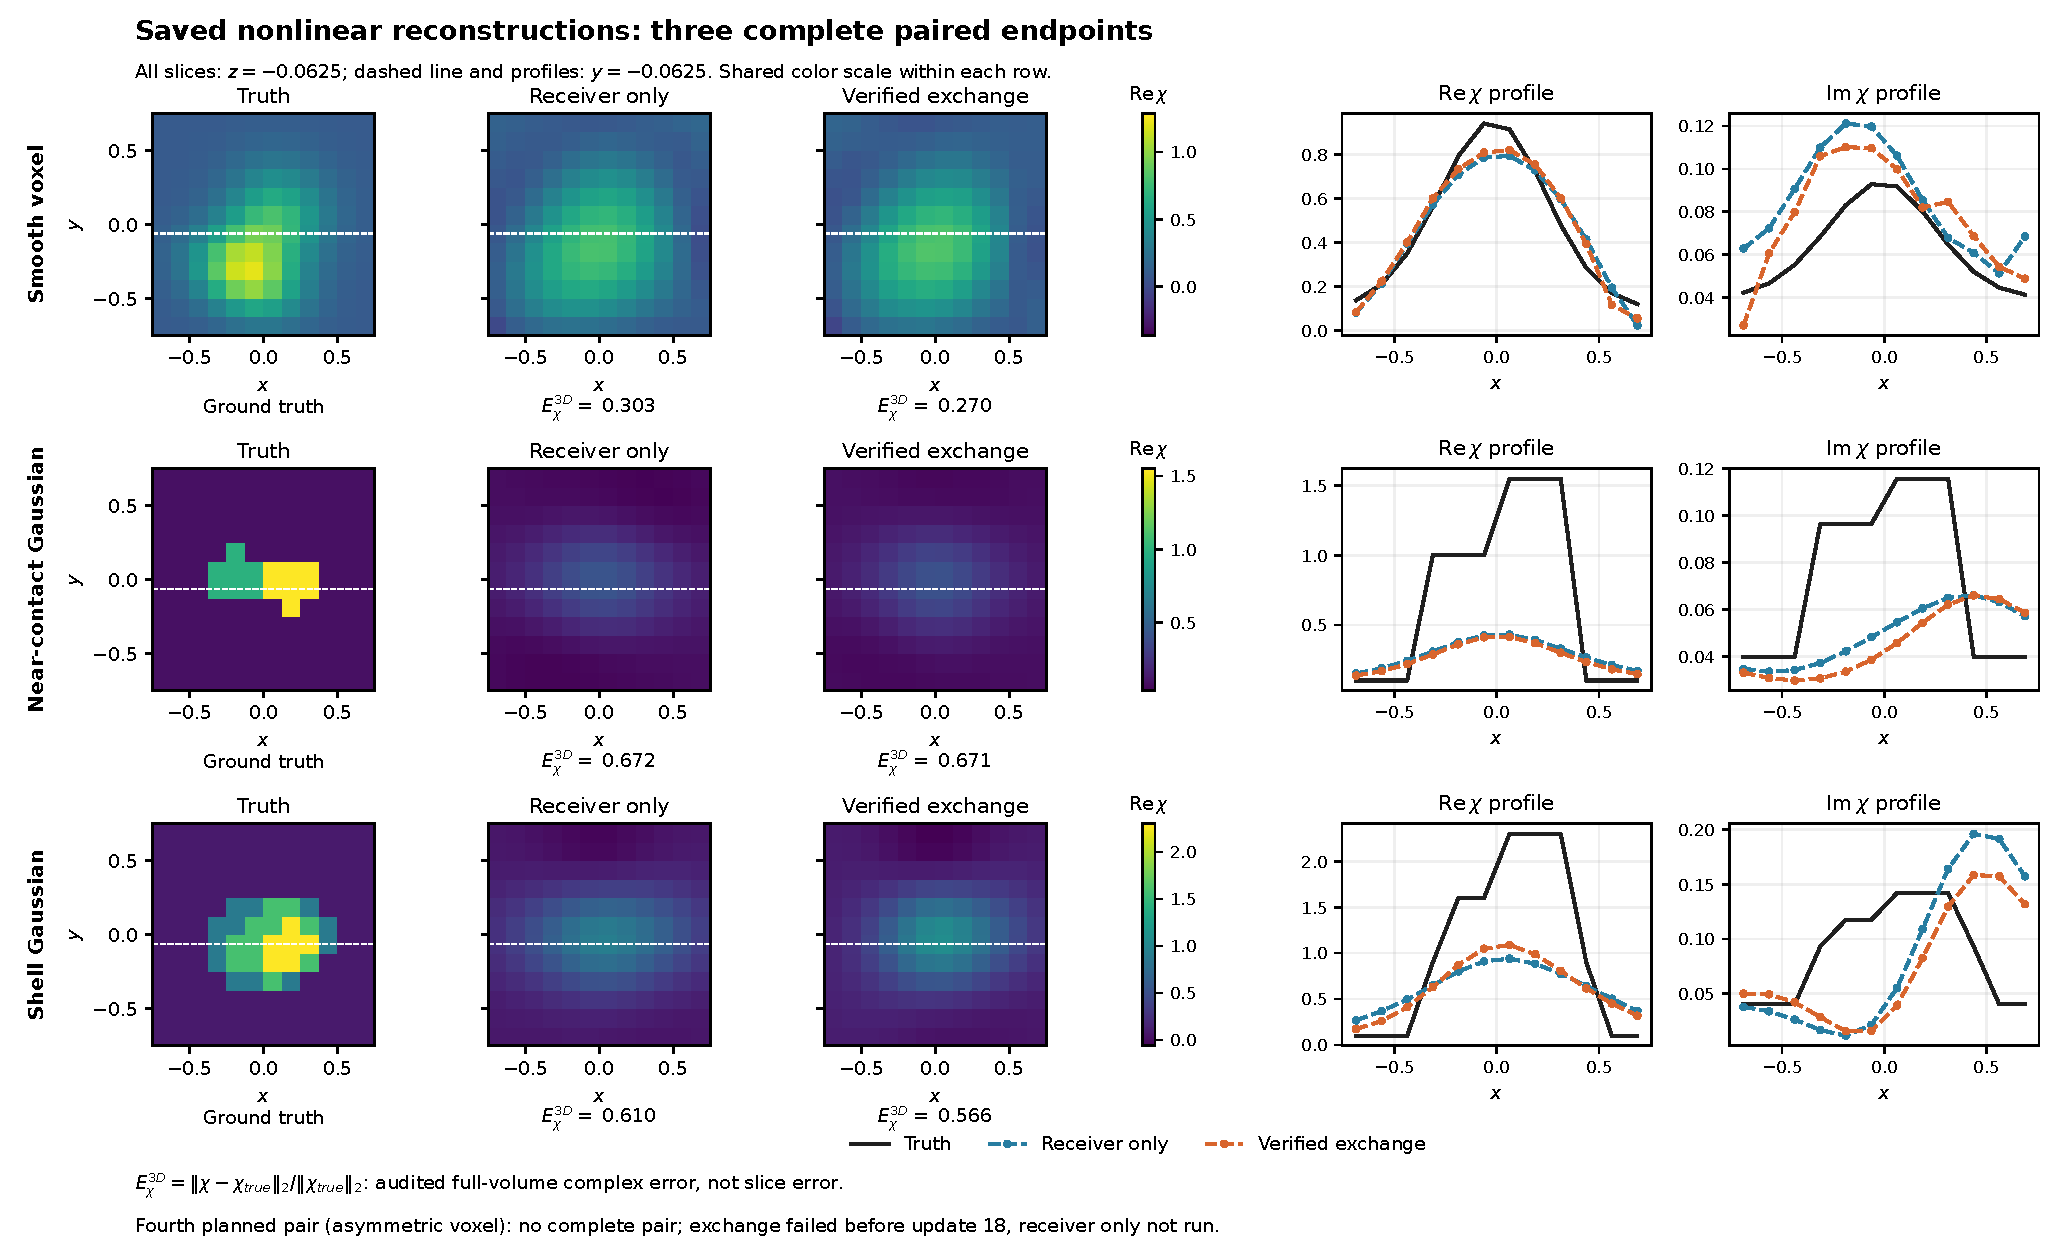
\includegraphics[width=.97\linewidth]{figures/nonlinear_closure_v1/nonlinear_reconstructions.pdf}
\caption{从左到右先看真实材料、receiver与exchange的同一中心切片，再看实部和虚部剖面线。每行统一色标，避免颜色范围不同制造视觉优势。整个体积上的误差见上表；切片仅帮助理解改善出现在哪里。接触与shell峰值仍被平滑，说明有限测量和材料表示仍限制恢复。}
\end{figure}

\begin{figure}[htbp]\centering
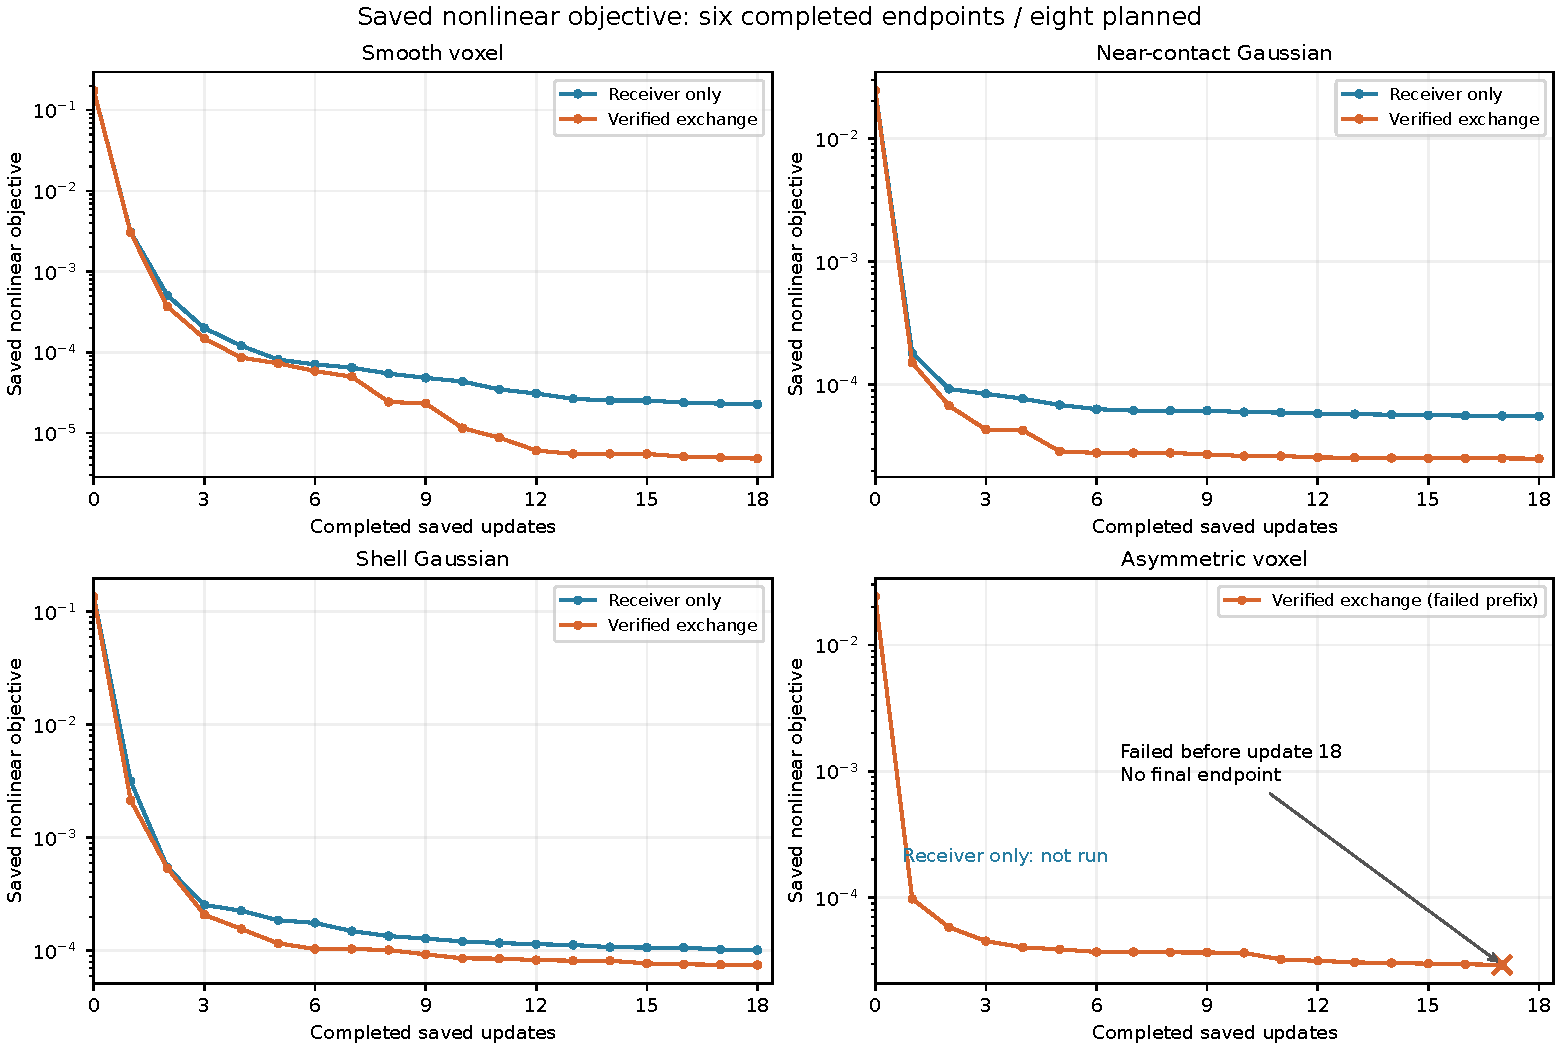
\includegraphics[width=.95\linewidth]{figures/nonlinear_closure_v1/nonlinear_objective_curves.pdf}
\caption{完整非线性目标（full nonlinear objective）随实际接受更新的变化。三个完整对照达到共同的18次更新上限。右下图单独保留非对称voxel的17步安全前缀，其后发生端点残差失败；没有对应的完成基线，不能把该曲线当作第四组成功。}
\end{figure}
